%%%%%%%%%%%%%%%%%%%% ANEXOS / APPENDIX %%%%%%%%%%%%%%%%%%%%%%
\appendix           % appendix starts from here
\appendixpage  		% add a blank page to start the appendix
\addappheadtotoc 	% add appendix to the TOC

\chapter{Software Implementation and Repository Structure}
\label{app:software_implementation}

This appendix describes the software implementation developed throughout the project. The complete implementation is organized as a modular repository covering the complete processing chain, from LiDAR data acquisition and packet processing to point cloud generation, dataset annotation, model training, and real-time semantic segmentation inference. The repository also contains dedicated tools for packet capture and replay, communication between the onboard and external processing units, model benchmarking, and dataset management.

The software was intentionally divided into independent components so that data acquisition, dataset generation, training, and inference could be developed and tested separately. This organization also enables recorded LiDAR data to be replayed without requiring the physical sensor and allows the inference system to operate independently from the acquisition hardware.

The complete source code developed for this work is available in the project repository.

\section{Repository Organization}
\label{sec:repository_organization}

The repository is organized into several groups of modules corresponding to the main stages of the proposed system. The principal structure is summarized below:

\begin{verbatim}
LiDAR/
|
|-- Data acquisition and processing
|   |-- main.py
|   |-- parser.py
|   |-- geometry.py
|   |-- streamer.py
|   |-- visualization.py
|   |-- pcd_writer.py
|   |-- pointcloud_saver.py
|   |-- config.py
|
|-- Packet capture and replay
|   |-- capture.py
|   |-- lidar_capture.py
|   |-- lidar_replay.py
|   |-- test_pcap.py
|   |-- lidar_packets.pcap
|
|-- Network communication
|   |-- sender.py
|   |-- receiver.py
|   |-- setup-daemon.sh
|   |-- start.sh
|
|-- Dataset generation and annotation
|   |-- dataset_anotator.py
|   |-- lidar_database/
|   |-- data_utils/
|
|-- Model inference
|   |-- inference/
|       |-- base_model.py
|       |-- inference_engine.py
|       |-- pcd_dataset.py
|       |-- metrics.py
|       |-- benchmark.py
|       |-- **model.py
|       |-- run_pointnet.py
|       |-- run_vector.py
|
|-- Model training
|   |-- finetunningPointnet.py
|   |-- finetunningPointnet2.py
|   |-- finetunningOpenpoints.py
|   |-- *.yaml
|
|-- Environment and checkpoints
|-- environment.yml
|-- checkpoints**/
|-- benchmark.csv
\end{verbatim}

The repository therefore contains not only the software required for final deployment, but also the tools developed during the intermediate stages of dataset construction, model development, and experimental evaluation.

\section{LiDAR Data Acquisition Software}
\label{sec:software_data_acquisition}

The data acquisition subsystem is responsible for receiving the raw Ethernet traffic generated by the LiDAR, decoding the sensor packets, reconstructing three-dimensional measurements, visualizing the resulting point cloud, and optionally storing the acquired data.

The main processing modules are distributed across \texttt{main.py}, \texttt{parser.py}, \texttt{geometry.py}, \texttt{streamer.py}, \texttt{visualization.py}, \texttt{pcd\_writer.py}, and \texttt{pointcloud\_saver.py}. This modular organization separates the network and packet-level processing from the geometric reconstruction and point cloud management.

\subsection{Application Entry Point}

The \texttt{main.py} module acts as the main entry point for the acquisition application. It coordinates the different components required to operate the LiDAR processing pipeline and provides the interface through which the acquisition system is configured and started.

The main application connects the packet acquisition stage with the subsequent processing modules. Consequently, the software can be operated as a complete real-time acquisition system without requiring the individual modules to be manually executed.

\subsection{Packet Parsing}

The \texttt{parser.py} module is responsible for interpreting the raw LiDAR packets received through the network interface. The parser extracts the binary payload generated by the sensor and converts the encoded measurements into structured information that can subsequently be processed geometrically.

This separation between packet parsing and geometric reconstruction allows the sensor-specific binary format to be isolated from the rest of the application. The resulting measurements can therefore be passed to the geometric processing stage without requiring the visualization or storage modules to directly manipulate raw Ethernet packets.

\subsection{Geometric Reconstruction}

The \texttt{geometry.py} module implements the conversion between the angular and range measurements provided by the LiDAR and the Cartesian coordinates used to construct the point cloud.

For each valid measurement, the corresponding distance and angular information are transformed into a three-dimensional point. The resulting coordinates constitute the common representation used by the subsequent visualization, storage, communication, and machine learning components.

This module therefore represents the interface between the sensor-specific measurement representation and the generic three-dimensional point cloud representation used throughout the remainder of the project.

\subsection{Real-Time Streaming and Visualization}

The \texttt{streamer.py} module manages the point cloud representation used during continuous acquisition. It provides access to the most recent reconstructed points and supports the temporal behavior required for real-time operation.

The visualization functionality is implemented separately through \texttt{visualization.py}. This separation allows point cloud acquisition to continue independently from the graphical visualization process. Consequently, visualization can be enabled during interactive acquisition or omitted during automated data collection when graphical output is unnecessary.

\subsection{Point Cloud Storage}

Point cloud storage is handled through dedicated modules rather than being implemented directly inside the packet processing code. The \texttt{pcd\_writer.py} module provides the functionality required to generate PCD files, while \texttt{pointcloud\_saver.py} manages the acquisition and saving of point clouds over time.

This separation allows the same reconstructed point cloud representation to be used simultaneously for visualization, storage, and network transmission. It also facilitates the generation of independent point cloud files that can subsequently be used during annotation and model training.

\section{Packet Capture and Replay}
\label{sec:software_capture_replay}

A separate subsystem was implemented to decouple software development and testing from the physical LiDAR sensor. The repository includes the \texttt{capture.py}, \texttt{lidar\_capture.py}, \texttt{lidar\_replay.py}, and \texttt{test\_pcap.py} modules, together with recorded packet data in PCAP format.

The capture functionality records the Ethernet traffic generated by the LiDAR and stores it in a PCAP file. These recordings preserve the original packet structure and provide a reproducible input for subsequent experiments.

The replay functionality reads the recorded packets and feeds them back into the processing pipeline. As a result, the parser and geometric reconstruction modules can be tested using identical input data across multiple experiments.

This mechanism was particularly useful during development because it allowed packet parsing, point cloud reconstruction, and downstream processing to be evaluated without continuously operating the physical sensor.

The use of a recorded PCAP also makes it possible to reproduce specific acquisition conditions when debugging the system. Errors in packet decoding or geometric reconstruction can therefore be investigated using a fixed input sequence rather than relying on a new physical acquisition for every test.

\section{Communication Between Acquisition and Inference}
\label{sec:software_communication}

The final deployment architecture separates LiDAR acquisition from neural network inference. Communication between both processing units is implemented through the \texttt{sender.py} and \texttt{receiver.py} modules.

\subsection{Point Cloud Sender}

The \texttt{sender.py} module is executed on the acquisition side and implements a TCP client responsible for transmitting reconstructed point clouds to the external processing computer.

The sender periodically obtains the current point cloud from the streaming component. Before transmission, the number of points is encoded as a four-byte unsigned integer, followed by the point coordinates stored as 32-bit floating-point values. The resulting message therefore contains both the size of the point cloud and the corresponding sequence of XYZ coordinates.

The sender also implements automatic reconnection. If the TCP connection is unavailable, the software periodically attempts to reconnect to the configured receiver. Similarly, if an active connection is interrupted during transmission, the socket is closed and the connection procedure is restarted.

This behavior allows the acquisition process to remain independent of the availability of the inference workstation.

\subsection{Point Cloud Receiver}

The \texttt{receiver.py} module implements the server side of the communication architecture. It listens for TCP connections on port 5005 and waits for a connection from the acquisition node.

Once a connection has been established, the receiver first reads a four-byte header containing the number of points in the incoming frame. It then reads the corresponding payload, which contains three 32-bit floating-point values for each point. The received byte sequence is converted into a NumPy array and reshaped into an $(N\times3)$ matrix representing the XYZ point cloud.

The resulting point cloud is passed directly to the inference engine through the \texttt{process()} method. The receiver therefore does not implement the neural network itself; instead, its responsibility is to provide the communication interface between the network and the inference subsystem.

This design keeps the network communication layer independent from the selected segmentation architecture and allows the inference implementation to be modified without changing the point cloud transmission protocol.

\subsection{Autonomous Startup}

The repository also contains \texttt{setup-daemon.sh} and \texttt{start.sh}, which support the automated initialization of the acquisition system.

These scripts are used to configure and start the required acquisition processes without requiring a graphical environment or manual interaction. This functionality is consistent with the headless operation described in the deployment architecture presented in Chapter~\ref{subsec:deployment_architecture}.

\section{Dataset Annotation and Data Management}
\label{sec:software_dataset}

The repository includes dedicated software for dataset organization and annotation. The main annotation application is implemented in \texttt{dataset\_anotator.py}, while additional data-management functionality is contained in the \texttt{data\_utils} directory.

The annotation software provides an interactive environment in which point clouds can be inspected and human regions can be selected. The implementation supports the annotation strategies described in Section~\ref{subsec:annotation}, including seed-based selection and geometric or clustering-based segmentation.

The resulting labels maintain correspondence with the original point ordering, allowing the point cloud and semantic annotation to be loaded independently while preserving their one-to-one relationship.

The \texttt{lidar\_database} directory contains the data associated with the acquisition and annotation stages. The separation between raw point cloud data, annotations, and processing utilities allows the same dataset to be reused across different training and evaluation experiments.

\section{Inference Software}
\label{sec:software_inference}

The inference subsystem is contained in the \texttt{inference} directory. It provides the components required to load trained models, prepare point cloud data, perform semantic segmentation, calculate evaluation metrics, and benchmark model execution.

The directory contains a common model interface through \texttt{base\_model.py}, the central \texttt{inference\_engine.py}, the point cloud dataset implementation in \texttt{pcd\_dataset.py}, the metric implementation in \texttt{metrics.py}, and a benchmarking module in \texttt{benchmark.py}. Individual model wrappers are provided for the evaluated architectures, including PointNet, PointNet++, DGCNN, PointNeXt-S, PointNeXt-XL, and PointVector.

\subsection{Inference Engine}

The \texttt{inference\_engine.py} module provides the central execution layer for inference. It receives a point cloud from the communication layer, prepares it for model execution, invokes the selected neural network, and returns the resulting prediction together with processing statistics.

The use of a dedicated inference engine prevents the receiver from becoming dependent on the internal implementation of a particular neural network. The communication system therefore interacts with a common processing interface rather than directly accessing model-specific functions.

This architecture makes it possible to replace the segmentation model while preserving the acquisition and communication components.

\subsection{Model Wrappers}

Each evaluated architecture has an associated model implementation inside the \texttt{inference} directory. These modules provide a common interface between the inference engine and the different network implementations.

The model wrappers are responsible for constructing the corresponding architecture, loading its trained parameters, configuring the execution device, and exposing the inference functionality required by the engine.

This organization is particularly useful because the evaluated architectures originate from different implementations and frameworks. A common abstraction layer allows them to be evaluated through the same inference pipeline while retaining their original implementations.

\subsection{Point Cloud Input Processing}

The \texttt{pcd\_dataset.py} module provides the data interface used to load point cloud files and prepare them for model processing. This component isolates file handling and input preparation from the neural network implementation.

The inference system operates on XYZ coordinates, matching the input representation adopted during the fine-tuning process. The resulting tensor representation is subsequently passed to the selected model for point-wise classification.

\subsection{Evaluation and Benchmarking}

The \texttt{metrics.py} module contains the evaluation functionality used to quantify segmentation performance. The repository also provides \texttt{benchmark.py}, which is used to evaluate computational behavior and execution performance.

The separation between inference and benchmarking allows the same trained models to be evaluated both functionally and computationally. This is particularly relevant for the objectives of this work, where segmentation quality must be considered together with the computational requirements of the candidate architectures.

\section{Model Training and Fine-Tuning}
\label{sec:software_training}

The training subsystem contains dedicated scripts for adapting the selected architectures to the custom UAV dataset. The repository includes separate fine-tuning programs for PointNet, PointNet++, and the OpenPoints-based architectures.

The principal training scripts are:

\begin{itemize}
\item \texttt{finetunningPointnet.py},
\item \texttt{finetunningPointnet2.py},
\item \texttt{finetunningOpenpoints.py}.
\end{itemize}

The OpenPoints-based training configuration is further specified through YAML files corresponding to DGCNN, PointNeXt-S, PointNeXt-XL, and PointVector.

\subsection{PointNet and PointNet++ Training}

PointNet and PointNet++ are trained through dedicated PyTorch scripts. These scripts implement the dataset loading, model initialization, transfer learning modifications, optimization, validation, and checkpoint generation required for the corresponding experiments.

The dedicated implementations were retained because these models were initially evaluated with the objective of determining whether lightweight architectures could be executed on the embedded platform.

\subsection{OpenPoints-Based Training}

The training of DGCNN, PointNeXt-S, PointNeXt-XL, and PointVector is organized around the OpenPoints framework. The repository contains architecture-specific YAML configuration files that define the parameters required by the corresponding training procedures.

This organization separates experiment configuration from the training implementation and makes it possible to reproduce different model configurations without modifying the core training code.

\subsection{Transfer Learning Adaptation}

The training code implements the modifications required to transfer models pretrained on S3DIS to the proposed binary UAV segmentation task.

The original models expect the feature representation associated with the S3DIS dataset. Since the acquired LiDAR data contain XYZ coordinates but no RGB information, the input representation is adapted to three-dimensional coordinates. Similarly, the original multi-class segmentation output is replaced by the binary Human/Background classification required by the proposed dataset.

Compatible pretrained parameters are retained, while parameters associated with the modified input and output layers are initialized for the target task. The complete network is subsequently fine-tuned using the UAV dataset.

\subsection{Training Outputs}

The training scripts generate trained model checkpoints that are subsequently used by the inference subsystem. The repository contains multiple checkpoint directories corresponding to the evaluated architectures, including PointNet++, DGCNN, PointNeXt-S, PointNeXt-XL, PointVector, and the PointNet-related experiments.

This organization establishes a direct connection between the training and deployment stages: the checkpoint generated during training can be loaded by the corresponding inference wrapper and subsequently used by the real-time receiver.

\section{Relationship Between Software Components}
\label{sec:software_pipeline}

The complete software system can therefore be understood as a sequence of interconnected but independent stages.

During online operation, the LiDAR generates raw Ethernet packets that are processed by the acquisition software. The packet parser extracts the measurements, the geometric processing module reconstructs the corresponding XYZ coordinates, and the streaming component maintains the current point cloud.

The point cloud is simultaneously available for visualization and storage and can be transmitted through the network sender. On the external processing computer, \texttt{receiver.py} reconstructs the transmitted point cloud from the TCP stream and passes it to the \texttt{InferenceEngine}. The inference engine prepares the input and invokes the selected trained model. The resulting point-wise predictions and processing statistics are then returned to the receiver.

The same software structure can also be used without the physical sensor. Recorded PCAP data can be replayed through the packet replay subsystem, allowing the acquisition and processing stages to be evaluated using previously captured measurements.

The training branch of the repository is largely independent from the online acquisition branch. Annotated PCD files are loaded by the training pipeline, processed according to the selected architecture, and used to generate model checkpoints. These checkpoints subsequently become inputs to the inference branch.

The overall relationship can be summarized as:

\begin{figure}
    \centering
    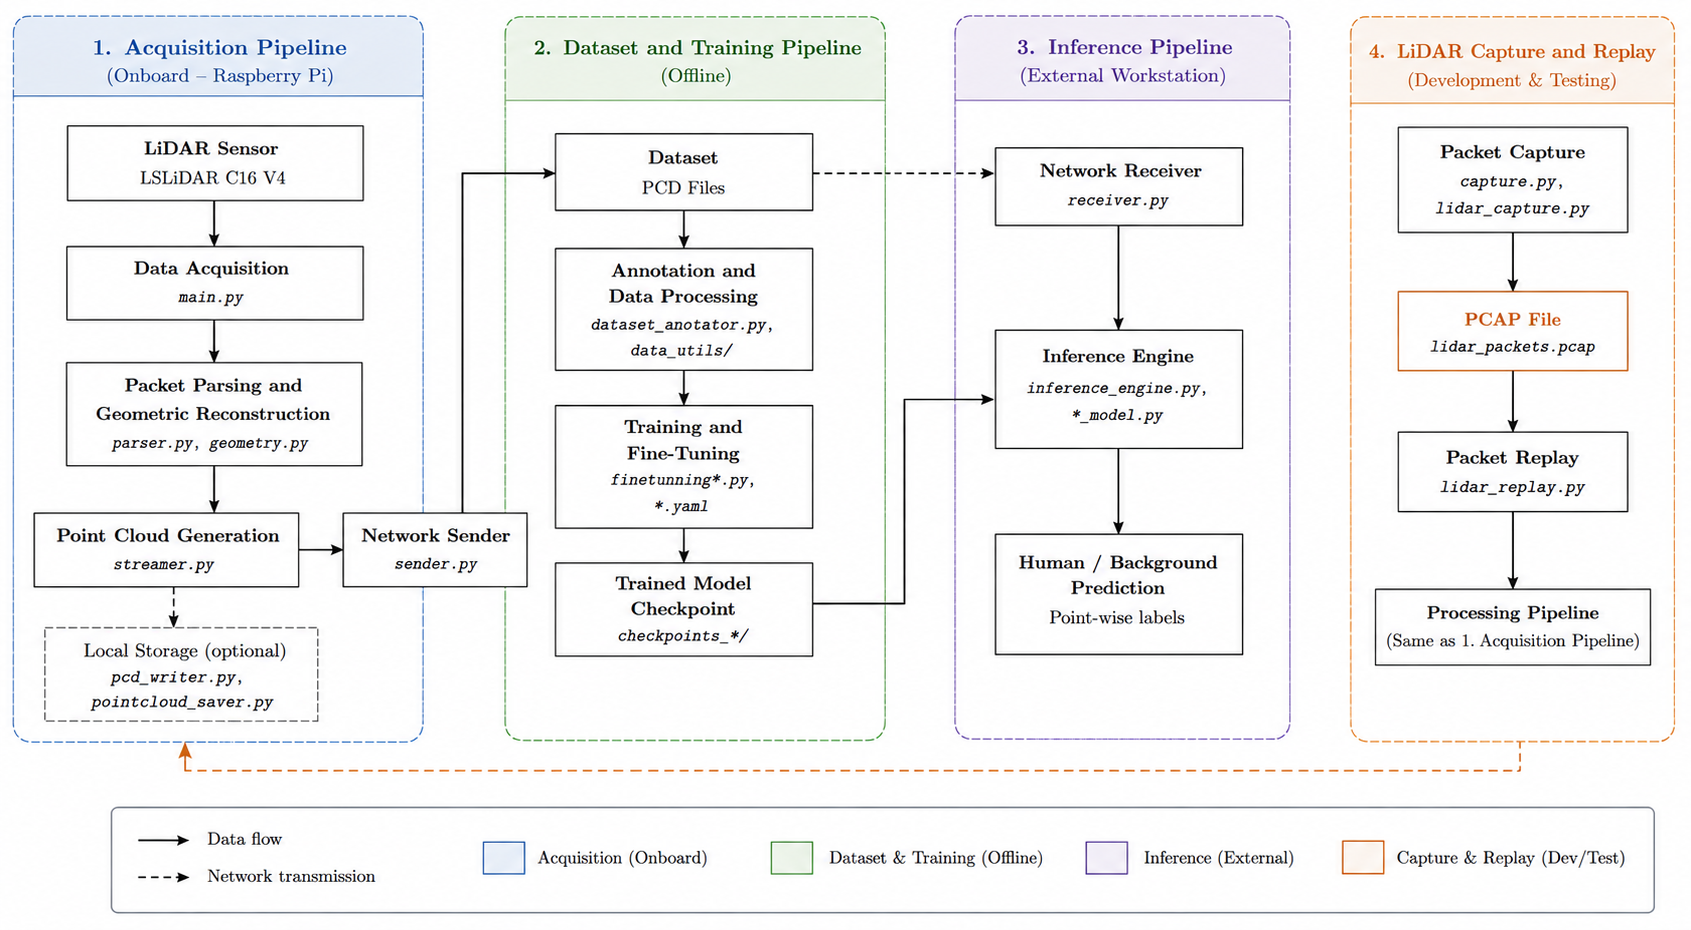
\includegraphics[width=1\linewidth]{code diagram.png}
    \caption{Relationship between the main software components developed for LiDAR
acquisition, dataset generation, model training, and semantic segmentation inference.}
    \label{fig:placeholder}
\end{figure}


The resulting architecture provides a complete software path from raw sensor measurements to semantic segmentation predictions while maintaining a clear separation between acquisition, communication, machine learning, and evaluation components.

\section{Reproducibility}
\label{sec:software_reproducibility}

The repository also contains the configuration and environment information required to reproduce the software environment. In particular, \texttt{environment.yml} specifies the Python environment used by the project, while the YAML configuration files provide the architecture-specific parameters used by the OpenPoints training experiments.

The inclusion of packet captures, dataset utilities, training scripts, model checkpoints, inference implementations, and benchmarking utilities provides a complete software record of the development process.

Rather than relying on a single monolithic application, the implementation is divided into reusable modules that can be individually tested. This modularity was especially important during development because the acquisition system, dataset generation process, training pipeline, and final inference system could be validated independently before being integrated into the complete deployment architecture.

Overall, the repository constitutes the software implementation accompanying the hardware platform and machine learning methodology described throughout this work. The main body of the thesis focuses on the design decisions and experimental methodology, while this appendix documents how those components are concretely implemented in software.


\chapter{Detailed Training Configuration}
\label{app:training_configuration}

This appendix provides the detailed configuration used for training and fine-tuning the semantic segmentation models evaluated in this work. The information presented here complements the general training methodology described in Section~\ref{subsec:training_configuration} and documents the parameters implemented in the training scripts and configuration files of the developed software framework.

\section{Training Software and Execution Environment}
\label{app:training_environment}

The training pipeline was implemented in Python using PyTorch. The repository contains separate training scripts for the PointNet and PointNet++ architectures, while the PointNeXt, DGCNN, and PointVector models are configured using the OpenPoints framework. The corresponding model configurations are stored in YAML files, allowing the architectural parameters to be separated from the training scripts.

The Python environment used by the project is based on Python 3.10. The repository environment configuration defines a dedicated Conda environment named \texttt{pointnet2}.

All training scripts automatically select CUDA when a compatible GPU is available and otherwise fall back to CPU execution. The training process also enables deterministic cuDNN behaviour by setting deterministic execution and disabling cuDNN benchmarking. A fixed random seed of 42 is used for Python, NumPy, and PyTorch random number generators.

\section{Dataset Split and Sampling}
\label{app:dataset_sampling}

The custom dataset is loaded through the \texttt{MyLidarDataset} class. Point cloud files are first sorted and then shuffled using a fixed random seed of 42. The resulting dataset is divided into three subsets according to the following proportions:

\begin{itemize}
\item 75% of the scenes for training,
\item 15% for validation,
\item 10% for testing.
\end{itemize}

The split is performed at scene level rather than at point level. Consequently, different samples generated from the same point cloud remain within the same subset, preventing information from the same scene from being directly shared between training and validation or test sets.

Each scene can generate multiple training samples. The dataset length is defined as twenty times the number of scenes in the corresponding split. During each access to a scene, a new subset of 4096 points is generated.

A class-aware sampling mechanism is used to increase the frequency of human-containing regions during training. If the scene contains points belonging to the human class, a probability of 0.7 is assigned to selecting a human point as the centre of the sampled region. The 4096 points closest to this randomly selected human point are then used as the input sample. With the remaining probability, points are sampled randomly from the complete point cloud. This implements the 70/30 class-aware versus random sampling strategy described in the main methodology.

\section{Data Augmentation}
\label{app:data_augmentation}

Data augmentation is applied only to the training split. The transformations are implemented directly in the dataset loader and are therefore applied online when each sample is generated.

The augmentation pipeline consists of four transformations that modify the point coordinates while preserving their semantic labels.

First, a random rotation around the vertical axis is applied. The rotation angle is sampled uniformly from the interval

$[
\theta \sim \mathcal{U}(0,2\pi).
]$

Second, a global scaling factor is sampled from

$[
s \sim \mathcal{U}(0.95,1.05),
]$

introducing small variations in the apparent scale of the scene.

Third, zero-mean Gaussian noise is added independently to the point coordinates. The standard deviation of the noise is 0.005.

Finally, a random translation is applied independently to the three coordinate axes, with each displacement sampled from the interval

[
[-0.02,0.02].
]

In addition, point dropout is applied with a probability of 0.3. When activated, approximately 10% of the sampled points are replaced by the first point in the sample. These transformations introduce variations in orientation, scale, position, measurement noise, and point density, thereby increasing the variability observed during training.

\section{Common Optimization Configuration}
\label{app:optimization}

The PointNet, PointNet++, and PointVector/PointNeXt/DGCNN training implementations use a common optimization strategy based on the AdamW optimizer. The optimizer parameters are

\begin{itemize}
\item $\beta_1 = 0.9$,
\item $\beta_2 = 0.999$,
\item $\epsilon = 10^{-8}$,
\item weight decay $=10^{-4}$.
\end{itemize}

The learning rate is architecture-dependent. The PointNet and PointNet++ training scripts use an initial learning rate of $10^{-4}$, whereas the PointVector/PointNeXt training script uses $10^{-3}$. The maximum number of training epochs is 100 and the batch size is 8 for all the corresponding training scripts.

A \texttt{ReduceLROnPlateau} scheduler is used to adapt the learning rate according to validation mIoU. The scheduler operates in maximization mode, reducing the learning rate by a factor of 0.5 after five consecutive validation evaluations without improvement. The minimum learning rate is limited to $10^{-7}$.

The optimization objective is a weighted cross-entropy loss. Two classes are considered: \textit{background} and \textit{person}. The corresponding class weights are 1.0 and 10.0, respectively, giving greater importance to the human class during optimization. An ignore index of $-100$ is used for invalid labels.

Gradient norm clipping is applied after backpropagation, with a maximum norm of 1.0. The training implementations using mixed precision employ PyTorch automatic mixed-precision execution and a \texttt{GradScaler} when CUDA is available.

\section{PointNet Configuration}
\label{app:pointnet_configuration}

PointNet is trained using the official PyTorch implementation. The training script loads the model through \texttt{models.pointnet\_sem\_seg} and configures it for two semantic classes. The input point cloud contains 4096 XYZ points per sample.

The training configuration is summarized in Table~\ref{tab:app_pointnet_config}.

\begin{table}[H]
\centering
\caption{PointNet training configuration.}
\label{tab:app_pointnet_config}
\begin{tabular}{|l|l|}
\hline
\textbf{Parameter} & \textbf{Value} \\
\hline
Implementation & Official PyTorch implementation \\
Number of classes & 2 \\
Input points & 4096 \\
Batch size & 8 \\
Maximum epochs & 100 \\
Initial learning rate & $1\times10^{-4}$ \\
Optimizer & AdamW \\
Weight decay & $1\times10^{-4}$ \\
Scheduler & ReduceLROnPlateau \\
Scheduler factor & 0.5 \\
Scheduler patience & 5 epochs \\
Minimum learning rate & $1\times10^{-7}$ \\
Class weights & [1.0, 10.0] \\
Gradient clipping & 1.0 \\
Early stopping patience & 20 epochs \\
Random seed & 42 \\
\hline
\end{tabular}
\end{table}

The training script evaluates validation loss, accuracy, mIoU, human IoU, human recall, and human F1-score after each epoch. The model achieving the highest validation mIoU is stored as the best checkpoint. Training is stopped when validation mIoU fails to improve for the configured patience period.

\section{PointNet++ Configuration}
\label{app:pointnet2_configuration}

PointNet++ follows the same general optimization strategy as PointNet. The model is loaded through the official PointNet++ semantic segmentation implementation and adapted to the two-class human/background task. The configuration uses 4096 input points, a batch size of 8, an initial learning rate of $10^{-4}$, and a maximum of 100 epochs.

The main parameters are summarized in Table~\ref{tab:app_pointnet2_config}.

\begin{table}[H]
\centering
\caption{PointNet++ training configuration.}
\label{tab:app_pointnet2_config}
\begin{tabular}{|l|l|}
\hline
\textbf{Parameter} & \textbf{Value} \\
\hline
Implementation & Official PyTorch implementation \\
Number of classes & 2 \\
Input points & 4096 \\
Batch size & 8 \\
Maximum epochs & 100 \\
Initial learning rate & $1\times10^{-4}$ \\
Optimizer & AdamW \\
Weight decay & $1\times10^{-4}$ \\
Scheduler & ReduceLROnPlateau \\
Scheduler factor & 0.5 \\
Scheduler patience & 5 epochs \\
Minimum learning rate & $1\times10^{-7}$ \\
Class weights & [1.0, 10.0] \\
Gradient clipping & 1.0 \\
Early stopping patience & 20 epochs \\
Random seed & 42 \\
\hline
\end{tabular}
\end{table}

The training and validation datasets use the same point sampling and augmentation mechanism described previously. The best checkpoint is selected according to validation mIoU. The implementation also supports loading compatible pretrained parameters while ignoring parameters whose names or tensor dimensions do not match the target architecture.

\section{OpenPoints-Based Architectures}
\label{app:openpoints_configuration}

PointNeXt-S, PointNeXt-XL, DGCNN, and PointVector are implemented using the OpenPoints framework. Their model-specific architectural configurations are stored in the files \texttt{pointnext-s.yaml}, \texttt{pointnext-xl.yaml}, \texttt{dgcnn.yaml}, and \texttt{pointvector.yaml}, respectively.

Unlike the PointNet and PointNet++ implementations, these configurations explicitly define four input channels. During training, the first three channels correspond to the XYZ coordinates, while an additional constant channel is appended to the input. For the PointVector implementation, the three-dimensional coordinates are supplied separately as positional information, while the four-channel representation is supplied as the feature tensor.

\subsection{PointNeXt-S}

The PointNeXt-S configuration uses a PointNeXt encoder with an initial width of 32 and five stages containing one block each. The encoder uses strides of

[
[1,4,4,4,4]
]

and two set-abstraction layers. Local neighbourhoods are constructed using ball queries with a radius of 0.1 and 32 neighbouring points. Feature aggregation uses the \texttt{dp\_fj} feature representation and max reduction. The decoder is implemented using \texttt{PointNextDecoder}, followed by a two-class segmentation head.

\subsection{PointNeXt-XL}

PointNeXt-XL uses a substantially larger encoder. Its five stages contain

[
[1,4,7,4,4]
]

blocks and use an initial width of 64. The configuration employs a single set-abstraction layer and does not use residual connections at this stage. As in PointNeXt-S, the neighbourhood radius is 0.1 and 32 neighbours are considered. The segmentation head produces two output classes. The YAML configuration specifies a batch size of 8.

The configuration file also reports a reference computational complexity of approximately 84.81 GFLOPs and 41.576 million parameters, together with a reported throughput of approximately 46.07 instances per second under the profiling configuration associated with the model. These values describe the reference configuration in the model file rather than measurements obtained during the experiments of this work.

\subsection{DGCNN}

The DGCNN configuration uses an EdgeConv-based encoder with five residual blocks. The network uses 64 channels, an embedding dimension of 1024, and $k=20$ neighbours for graph construction. The segmentation head contains MLP layers with dimensions 512 and 256 and produces two output classes. The configured batch size is 8.

The configuration file also contains reference profiling information for the OpenPoints implementation. It reports approximately 90.41 GFLOPs, 1.278 million parameters, and a reference throughput of approximately 8.02 instances per second for one of the profiling configurations. These values are framework profiling results and are therefore not used as experimental latency measurements in this work.

\subsection{PointVector}

PointVector uses the PointVector encoder with the same five-stage block configuration as PointNeXt-XL,

[
[1,4,7,4,4],
]

and an initial width of 64. The encoder uses 32 neighbours within a ball-query radius of 0.1. The configuration specifies \texttt{flag=1}, corresponding to the S3DIS configuration used by the model implementation. The decoder is implemented using \texttt{PointVectorDecoder}, and the segmentation head produces two classes. The configured batch size is 8.

\section{Summary of Model-Specific Parameters}
\label{app:training_summary}

Table~\ref{tab:app_training_summary} summarizes the principal parameters used across the evaluated architectures.

\begin{table}[H]
\centering
\caption{Summary of model-specific training configurations.}
\label{tab:app_training_summary}
\resizebox{\textwidth}{!}{
\begin{tabular}{|l|c|c|c|c|c|c|}
\hline
\textbf{Parameter} &
\textbf{PointNet} &
\textbf{PointNet++} &
\textbf{DGCNN} &
\textbf{PointNeXt-S} &
\textbf{PointNeXt-XL} &
\textbf{PointVector} \\
\hline
Input points & 4096 & 4096 & 4096 & 4096 & 4096 & 4096 \\
\hline
Batch size & 8 & 8 & 8 & 8 & 8 & 8 \\
\hline
Maximum epochs & 100 & 100 & 100 & 100 & 100 & 100 \\
\hline
Initial learning rate &
$10^{-4}$ &
$10^{-4}$ &
$10^{-3}$ &
$10^{-3}$ &
$10^{-3}$ &
$10^{-3}$ \\
\hline
Optimizer & AdamW & AdamW & AdamW & AdamW & AdamW & AdamW \\
\hline
Weight decay & $10^{-4}$ & $10^{-4}$ & $10^{-4}$ & $10^{-4}$ & $10^{-4}$ & $10^{-4}$ \\
\hline
LR scheduler & RLOP & RLOP & RLOP & RLOP & RLOP & RLOP \\
\hline
Scheduler patience & 5 & 5 & 5 & 5 & 5 & 5 \\
\hline
Early stopping & 20 & 20 & 20 & 20 & 20 & 20 \\
\hline
Classes & 2 & 2 & 2 & 2 & 2 & 2 \\
\hline
\end{tabular}
}
\end{table}

Here, RLOP denotes \texttt{ReduceLROnPlateau}. The learning-rate values shown for the OpenPoints-based architectures correspond to the training script configuration used in the repository, while the YAML files define the architecture-specific model parameters. The OpenPoints YAML files additionally specify a four-channel model input, while the training script constructs this representation from the XYZ coordinates by appending a constant feature channel.

\section{Checkpointing and Model Selection}
\label{app:checkpointing}

During training, checkpoints are generated to preserve both the latest training state and the best-performing model. The saved information includes the model parameters, optimizer state, scheduler state, validation mIoU, validation loss, and the corresponding training epoch.

The best model is selected according to validation mIoU. Whenever a new maximum validation mIoU is obtained, the model is stored as \texttt{best\_model.pth}. A separate \texttt{latest\_model.pth} file is also updated after each epoch, allowing training to be resumed from the latest available state.

Training terminates either when the maximum number of epochs is reached or when the validation mIoU has failed to improve for the configured early-stopping patience of 20 epochs. This mechanism is implemented in the PointNet, PointNet++, and PointVector/PointNeXt training scripts.

\section{Evaluation Metrics}
\label{app:evaluation_metrics}

The training scripts compute segmentation metrics from an accumulated point-wise confusion matrix. For the binary task, the reported metrics include global accuracy, per-class Intersection over Union (IoU), mean Intersection over Union (mIoU), precision, recall, and F1-score.

For each class, the IoU is computed as

$[
IoU_c =
\frac{TP_c}
{TP_c + FP_c + FN_c}.
]$

The mean Intersection over Union is then obtained as the arithmetic mean of the class-wise IoUs:

$[
mIoU =
\frac{1}{C}
\sum_{c=1}^{C} IoU_c,
]$

where $C=2$ for the binary human/background segmentation problem.

The human-class metrics are explicitly reported during validation because detecting the human class is the principal objective of the proposed system. The training scripts therefore report human IoU, human recall, and human F1-score in addition to the global validation metrics.
